\chapter{Quality Measures}

This chapter describes the various quality measures that were put in place to make sure that the code is as clean as possible and working as expected.

\section{Coding Guidelines}

\begin{itemize}
    \item General
    \begin{itemize}
        \item Code needs to be committed frequently with descriptive commit messages.
        \item Side effects should be avoided whenever possible.
        \item Comments may only be used if they are helpful.
        \item Global variables should be avoided if possible.
        \item Exceptions are preferred over error codes.
        \item Nesting should not be deeper than 2 levels.
        \item No duplicate code. (DRY)
        \item Functions should be kept short (less than 11 lines).
    \end{itemize}
    \item Formatting
    \begin{itemize}
        \item Line length should not exceed 120 characters.
    \end{itemize}
\end{itemize}

\section{Test Concept}

Due to the limited amount of time available, a proper test concept could not be created.
However, to ensure that the most important functionalities (i.e. the stepping functionalities) work,
some tests have been created.

The test log can be seen in \ref*{fig:testlog}.
For the testing, the \href{https://hackage.haskell.org/package/hspec}{hspec} package has been used.

\subsection{Unit Tests}
The \texttt{caseSpec}, \texttt{deltaSpec}, and \texttt{betaSpec} suites perform unit tests on the respective reduction functions.
These tests make sure that the reduction functions operate as expected.

\subsection{System Tests}
The \texttt{resultSpec} suite contains some system tests that compare the output of some test functions to the expected output.
These tests make sure that the reductions happen as expected.

\subsection{Difficulties during Testing}
During the testing process, some difficulties were encountered.
The main problem is that the identifiers for \texttt{Var}s are not always the same.
They can change between the execution of tests,
which makes the tests not repeatable.

To fix this issue,
instead of doing a full comparison,
only the parts between the \texttt{Var}s are compared.
The whole term is still tested,
but it is broken up into smaller comparisons instead of one large comparison comparing the whole term.

\begin{figure}[!ht]
    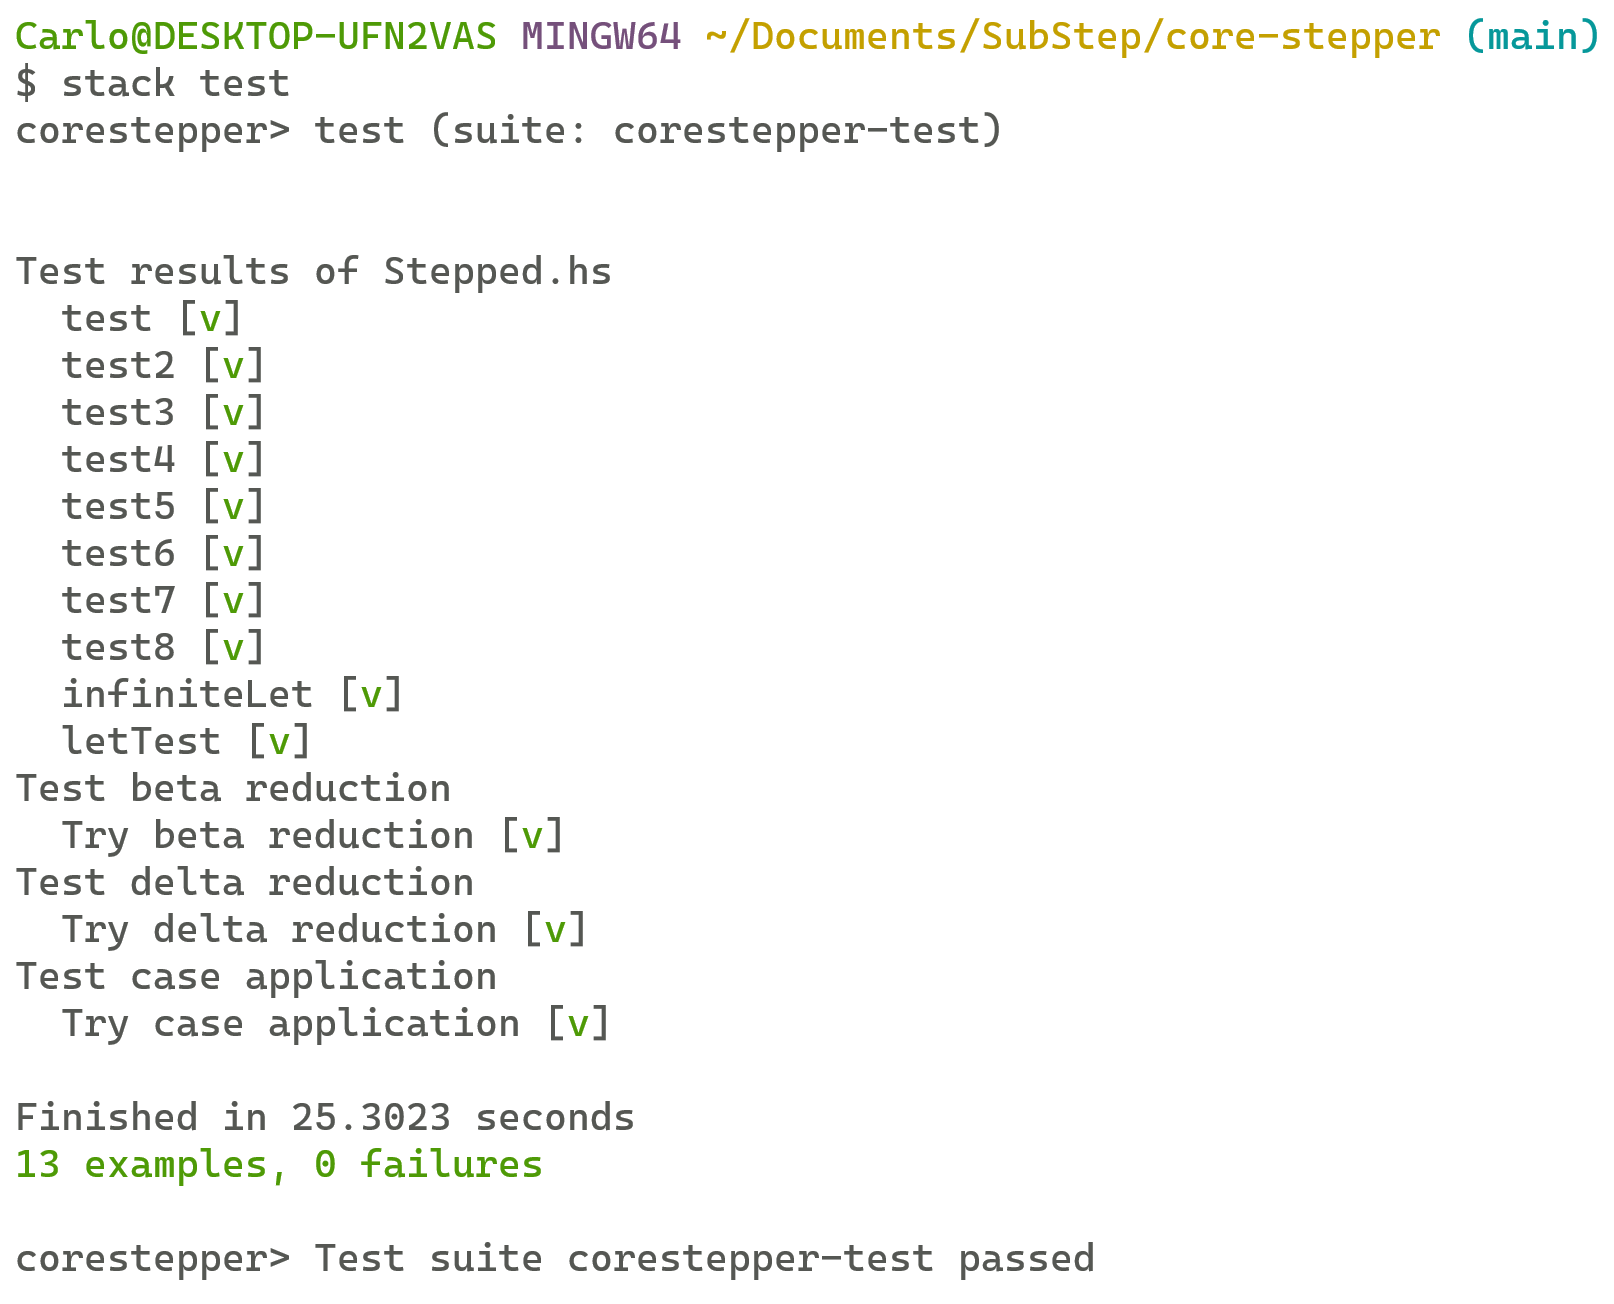
\includegraphics[width=0.75\textwidth]{resources/Tests.PNG}
    \caption{The test log}
    \label{fig:testlog}
\end{figure}
